% !TEX root = ../main.tex
\chapter{Solution}
\label{chapter:solution}

As stated on subsection \ref{subsection:rfc2000}, there is no mechanism to
decide if two constant expressions are equal. On this chapter,
we introduce \textsc{sire}, a symbolic executor for Rust, this provides a
framework to treat constant expression equality and in consequence to typecheck
programs with generics over constants. 

\section{Symbolic execution of Rust programs}

\textsc{sire} is an interpreter for the \textsc{mir} of Rust integrated with
the compiler. After the compiler generates the \textsc{mir}
for a function, \textsc{sire} takes this representation and executes it into
an small symbolic intermediate representation or \textsc{sir} for short.

Currently \textsc{sire} can only execute an small subset of all possible
functions. Specifically, it can execute functions without mutable arguments nor
mutable references as arguments containing the following subset of \textsc{mir}:

\begin{itemize}
    \item Statements: \texttt{Assign}, \texttt{StorageLive} and \texttt{StorageDead}.
    \item Terminators: \texttt{Goto}, \texttt{Return}, \texttt{Call} and \texttt{SwitchInt}.
    \item Rvalues: \texttt{BinaryOp}, \texttt{Ref} and \texttt{Use}.
    \item Operands: \texttt{Move}, \texttt{Copy} and \texttt{Constant}.
\end{itemize}

In addition, \textsc{sire} only supports integer and boolean types. Support for
structures, tuples, enumerations and arrays is planned in the future. Floating
point types are not supported given that they lack of the structural equality
property. \footnote{This was stated on
\href{https://github.com/rust-lang/rfcs/blob/master/text/1445-restrict-constants-in-patterns.md}{RFC-1445}.}


\subsection{Symbolic intermediate representation}

\textsc{sir} is a relatively simple language. Functions are the main construct
of \textsc{sir} and function arguments are numbered following the same
convention as \textsc{mir} where the zeroth argument is the return place.  The
grammar for \textsc{sir} can be found on \ref{lst:sir_grammar}.

The body of each function is composed of expressions which can be function
applications, binary operations, switch statements or pure values. 

There are only three kinds of values: Function arguments, constants and
function names. 

Finally, switch statements are composed by the value to be compared, the
possible values that it can take, and the result for each possible value (there
must be always a default result). 

 As an example, when executing the code on \ref{lst:rust_sire_example}, the
 \textsc{mir} and \textsc{sir} generated can be found on
 \ref{lst:mir_sire_example} and \ref{lst:sir_sire_example}.

\begin{listing}[ht]
    \begin{minted}{ebnf}
    defun   = '(defun' name {ty} expr ')';
    expr    = value | '('expr {expr}')' | '('op expr expr')' | 
             '(switch' expr {'('expr '->' expr')'} defcase);
    value   = '_'num | 'const' num | name;
    defcase = '(else ->' expr')';
    ty      = '(int' num')' | '(uint' num')' | 'bool';
    num     = ? a positive integer ?;
    name    = ? an string denoting the name of a function ?;
    op      = ? a binary operator ?;
    \end{minted}
    \caption{\textsc{sir}'s grammar in EBNF}
  \label{lst:sir_grammar}
\end{listing}

\begin{listing}[ht]
    \begin{minted}{rust}
    fn distance(x: i32, y: i32) -> i32 {
        if x > y {
           x - y
        } else {
           y - x
        }
    }
    \end{minted}
    \caption{A simple Rust function to be executed using \textsc{sire}}
  \label{lst:rust_sire_example}
\end{listing}

\begin{figure}[ht]
    \centering
    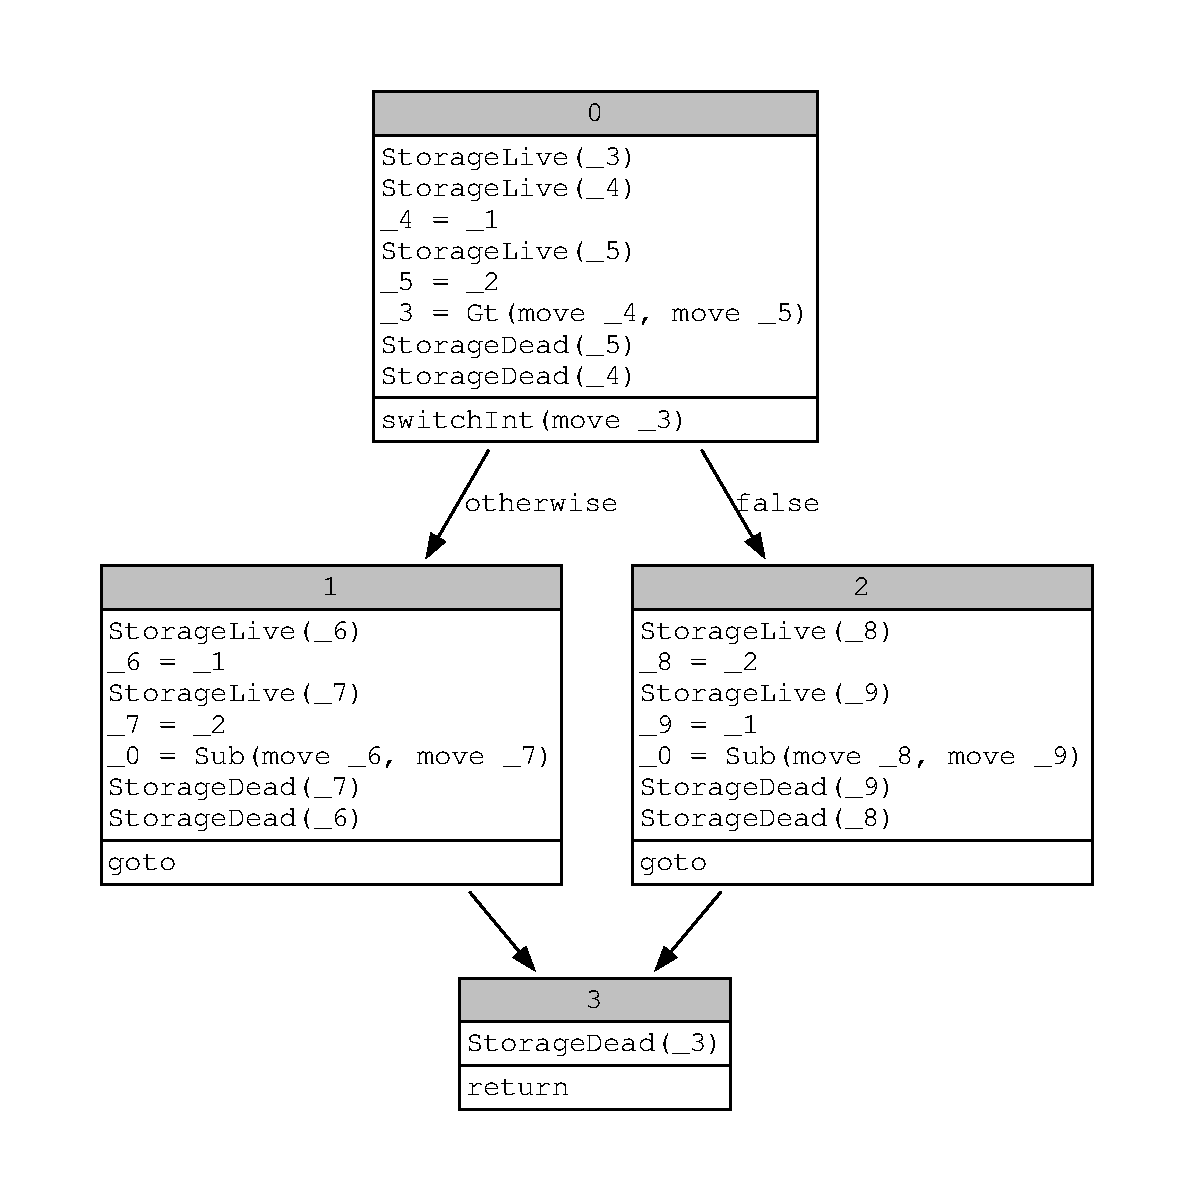
\includegraphics[height=12cm]{images/distance.pdf}
    \caption{The \textsc{mir} of the \texttt{distance} function on \ref{lst:rust_sire_example}}
  \label{lst:mir_sire_example}
\end{figure}

\begin{listing}[ht]
    \begin{minted}{lisp}
    (defun distance (int 32) (int 32) (int 32) 
        (switch (> _1 _2) 
            ((const 0) -> (- _2 _1)) 
             (else -> (- _1 _2))))
    \end{minted}
    \caption{The \textsc{sir} of the \texttt{distance} function on \ref{lst:rust_sire_example}}
  \label{lst:sir_sire_example}
\end{listing}

\begin{listing}[ht]
    \begin{minted}{lisp}
    (define-fun distance 
     ((x1 (_ BitVec 32)) (x2 (_ BitVec 32))) (_ BitVec 32) 
     (ite (bvsgt x1 x2) (bvsub x1 x2) (bvsub x2 x1)))
    \end{minted}
    \caption{The \texttt{smt-lib} snippet for the \textsc{sir} of the \texttt{distance} function on \ref{lst:rust_sire_example}}
  \label{lst:smt_sire_example}
\end{listing}


\subsection{Equality of symbolic functions}

Two \textsc{sir} functions are considered equal if they evaluate to the same
expression for every possible argument. For simple arithmetic expressions, this
can be achieved via E-unification. However, \textsc{sir} functions contain
control flow operations and recursive calls, in this case a theorem prover such
as Z3 is up to the task. \textsc{sire} can transform every \textsc{sir}
function into an small snippet in the \texttt{smt-lib} format to use it in an SMT.

Integer types on \textsc{sir} are transformed into \texttt{smt-lib} bit vectors
and the corresponding signed or unsigned arithmetic operations are used accordingly.
Switch expressions are transformed into nested conditionals. An example of such
snippets can be found on \ref{lst:smt_sire_example}. 

To decide if two functions are equal, is enough to write an small
\texttt{smt-lib} checking if the two functions are equal in their whole range. On \ref{lst:func_equality}, the \texttt{distance} function is compared with an alternative implementation found on \ref{lst:alt_distance}. 

\begin{listing}[ht]
    \begin{minted}{rust}
    fn alt_dist(x: i32, y: i32) -> i32 {
        let sign: i32; 
        if x > y {
           sign = 1;
        } else {
           sign = -1;
        }

        sign * (x - y)
    }
    \end{minted}
    \caption{An alternative implementation of the \texttt{distance} function on \ref{lst:rust_sire_example}}
  \label{lst:alt_distance}
\end{listing}

\begin{listing}[ht]
    \begin{minted}{lisp}
    (define-fun distance 
     ((x1 (_ BitVec 32)) (x2 (_ BitVec 32))) (_ BitVec 32) 
     (ite (bvsgt x1 x2) (bvsub x1 x2) (bvsub x2 x1)))

    (define-fun alt_dist 
     ((x1 (_ BitVec 32)) (x2 (_ BitVec 32))) (_ BitVec 32) 
     (ite (bvsgt x1 x2) 
      (bvmul (_ bv1 32) (bvsub x1 x2)) 
      (bvmul (_ bv4294967295 32) (bvsub x1 x2))))
    
    ;; Check it the functions are equal
    (assert (forall ((x1 (_ BitVec 32)) (x2 (_ BitVec 32))) 
     (= (distance x1 x2) (alt_dist x1 x2)))) 

    (check-sat) ;; sat
    \end{minted}
    \caption{equality check between the \texttt{distance} and \texttt{alt\_dist} functions}
  \label{lst:func_equality}
\end{listing}

\section{Typechecking of generics over constants}

\section{Generic traits over constants}

\begin{listing}[ht]
	\begin{minted}{rust}
    impl<'a, 'b, A: Sized, B, const N: usize> PartialEq<[B; N]> 
    for [A; N] where A: PartialEq<B> {
        fn eq(&self, other: &[B; N]) -> bool {
            self[..] == other[..]
        }
        fn ne(&self, other: &[B; N]) -> bool {
            self[..] != other[..]
        }
    }
	\end{minted}
    \caption{Implementing the \texttt{PartialEq} trait for all array sizes}
  \label{lst:trait_const_generics}
\end{listing}

\section{Bounds for generics over constants}

\begin{listing}[ht]
	\begin{minted}{rust}
    fn head<T, const N: usize>(array: [T; N]) -> T
    where {N > 0} {
        array[0]
    }
    \end{minted}
    \caption{Type-safe access to the first element of an array without using
    \texttt{Option<T>}}
  \label{lst:head_const_generics}
\end{listing}
\section{Validation}

In order to show that such extensions to Rust improve the ergonomy of the
language, an small library for numerical computing with and without our extended
syntax will be written. For both libraries, their cyclomatic complexity will be
computed and compared against each other. Given that these extensions to the
language remove some uses of control flow, a smaller complexity is expected.
